\documentclass{article}

\usepackage{amsmath,amssymb,amsthm,graphicx,setspace}
\usepackage[margin=1in]{geometry}
\usepackage[longnamesfirst]{natbib}
\bibliographystyle{ecta}
\newtheorem{theorem}{Theorem}
\onehalfspacing
\usepackage{enumerate}
\usepackage[table]{xcolor}
\usepackage{titlesec}
\usepackage{booktabs}
\usepackage{placeins} % for fixing table positions using \FloatBarrier

\setlength\parindent{0pt}

\title{AAA \\
    \normalsize BBB}
\date{\today}
\author{Your Name \\
        Email Adress}

\begin{document}

\maketitle

\begin{enumerate}[I]

%--- I ---%
\item \textbf{Single-Variable Linear Probability Model and Probit Models}

% including and referring to an equation
This refers to equation \ref{eq:struct}:

\begin{equation}\label{eq:struct}
    \beta_y y_t' + \gamma_z z_t' = \zeta_t
\end{equation}

% including table 
%\input{graphs/NullRejection}
%\FloatBarrier

% example: including a figure
\begin{figure}
    \centering
    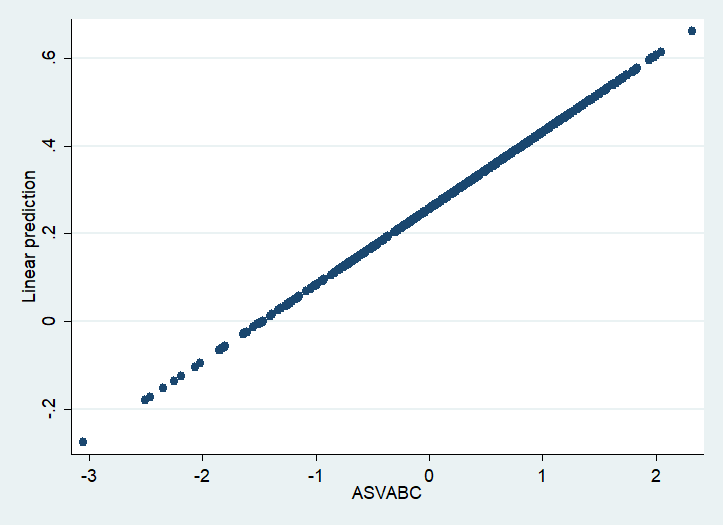
\includegraphics[scale = 0.15]{graphs/linear.png}
    \label{XXX}\caption{XXX}
\end{figure}
\FloatBarrier

\begin{enumerate}[1.]
    \item Answer to I.1
    
    \item \dots
    
    \item Answer to I.9
\end{enumerate}

%--- II ---%
\item\textbf{Multiple-Variable Logit Model}

\dots

%--- III ---%
\item\textbf{Estimating the Human Capital}

\dots

%--- IV ---%
\item\textbf{MLE}

\dots

\end{enumerate}
\end{document}

